% !TEX root = ../main.tex
\chapter{Overview of the Approach}
\label{chap:overview-of-the-approach}

In this chapter I introduce the high-level architecture overview of the proposed framework. The chapter also discusses each component in detail including details on how they cooperate.

\section{Architecture}
\label{sect:architecture}
\Cref{fig:architecture-overview} shows the overview of the framework's architecture. Since the novelty of the approach is how the source code representation is handled --- stored, transformed, and queried --- the heart of the approach is visualized on the right half of the figure. This is embedded and utilized in the framework itself, and integrated into the continuous integration circle and user-facing systems.

\begin{figure}[!htb]
  \centering
  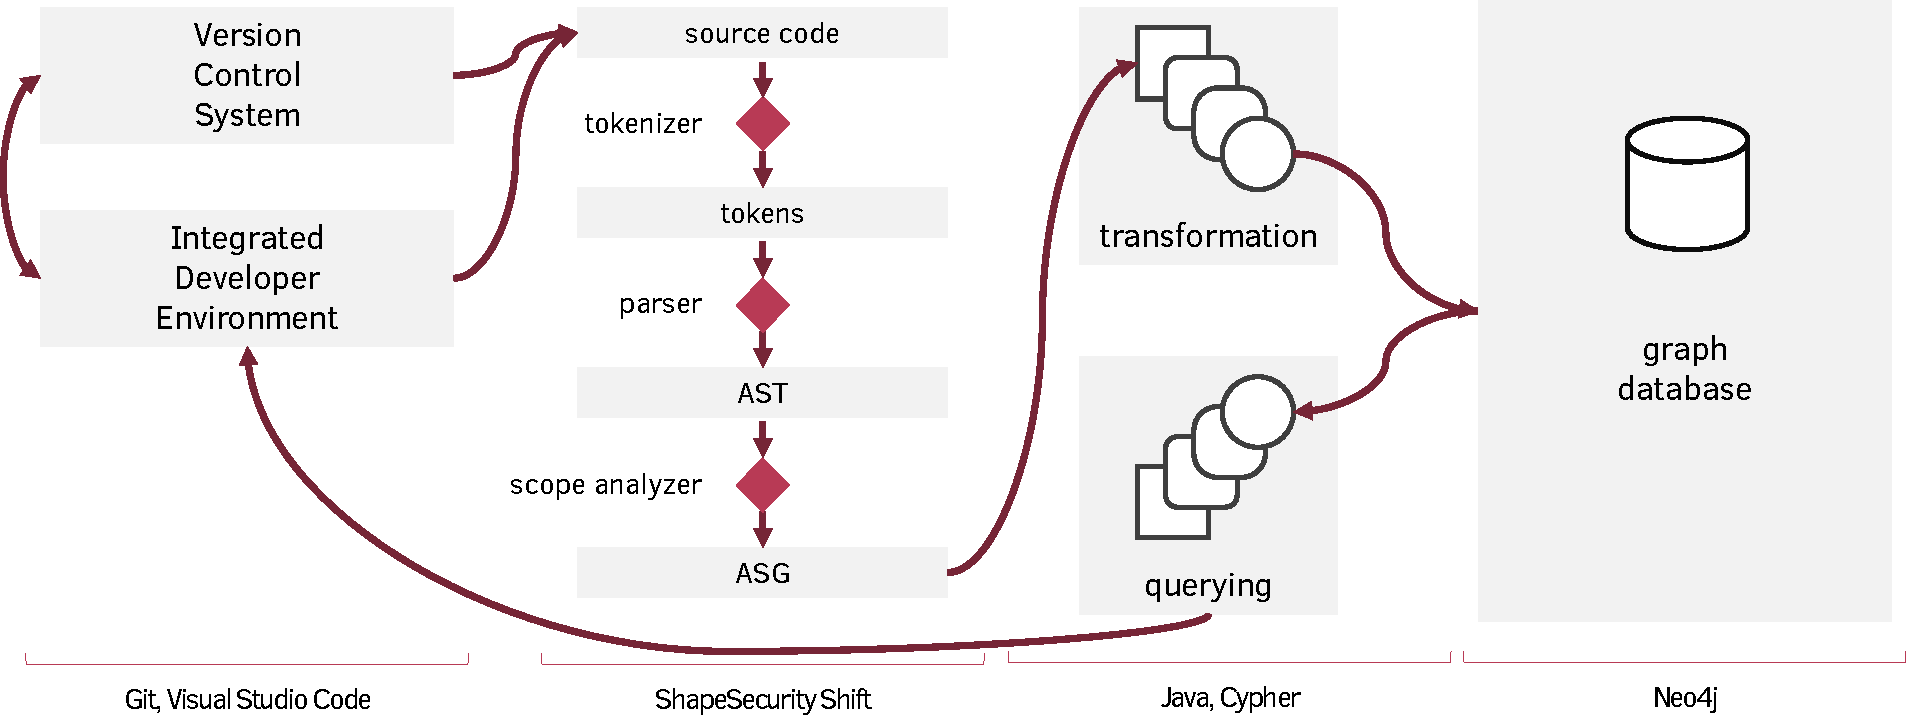
\includegraphics[width=\textwidth]{architecture-PPT.pdf}
  \caption{Architecture overview of the approach.}
  \label{fig:architecture-overview}
\end{figure}
% TODO update
% TODO add edge labels


\section{Main Components}
% TODO intro text (maybe the difference between this, steps of processing and the enumeration)

\subsection{Workflow Integration Points}
The framework is intended to be integrated with at least two types of development tooling. First, connecting to the \emph{Version Control System} makes it possible to extend the continuous integration workflow and provide the users of the system with current information about the codebase they are working on. Second, connecting to the \emph{Integrated Development Environment} empowers their users with feedback on the current modifications.

\subsubsection{Version Control System (VCS)}
Version control systems are change management systems for files (e.g., documents, software code). They store revisions of the current set of files managed by the system. Each revision is differentiated with a timestamp and also the person performing the changes are associated with a revision.

Version control is one of the most essential collaboration tools. When developers work on the same codebase, especially when the codebase is large, they need to share the code and work on it at the same time. Using a VCS, one can investigate the current version of the codebase at a selected revision. Also, it is possible to determine the changes performed between two revisions, manage multiple development branches with the same root and merge the changes made in these.

Integrating a VCS into the architecture makes it possible to extend the workflow with the features of the framework. By automatically calculating the changeset and forwarding this information to the framework, it is possible to keep an up-to-date representation of the version controlled data source.

The most known implementations are Git~\cite{git}, Subversion (SVN)~\cite{svn}, Mercurial (Hg)~\cite{hg}.

\subsubsection{Integrated Development Environment (IDE)}
An IDE is an application for (software) developers that integrates several tools making it easier to write, compile, and test the product. Integrated development environments are detailed in \Cref{sect:IDE}.

In the architectural overview, the IDE also represents the working set of the software and its dependencies available on the developer's computer. This working set also contains the developer's modifications that are not yet transferred to the shared VCS.
% TODO clarify, rephrase


\subsection{Transforming the Source Code}
\label{sect:overview-transforming-the-source-code}
One of the most important third party components of the approach is the source code parser. This component is used to transform a given source file, a \emph{compilation unit} into a model representation of the syntax and semantics of the source code. The process itself is detailed in~\Cref{sect:source-code-processing}.

A source code parsing toolkit with the following traits makes it possible to integrate it into the framework with ease:

\begin{itemize}[topsep=0pt]
  \item Provide the Abstract Syntax Tree and Abstract Semantic Graph for the parsed source file.

  \item Also provide scoping information
  % TODO

  \item Source code position
  % TODO

  \item Metamodel for the representation
  The more detailed metamodel, the better.
\end{itemize}

Since the \emph{Shape Security Shift} toolkit (detailed in~\Cref{sect:shift}) suits these requirements well, I have used the Java implementation of the \emph{Shift Parser}, and \emph{Scope Analyzer}.


\subsection{Graph Maintenance}
The novelty of my approach is how it processes, stores and connects the source code representation in a graph database. In this section I'll discuss how the subgraphs of the source code files are prepared and then connected to each other constructing a connected graph representing the whole source code repository.

The process can be summarized in 4 concise sentences:
\begin{enumerate}[topsep=0pt]
  \item The repository is transformed one file-by-file.
  \item The ASG \emph{model} is transformed into a \emph{property graph}.
  \item After every file is processed, the ASG subgraphs are interconnected using graph transformations.
  \item In case a file is added/modified/deleted, the corresponding subgraph is also added/removed and reprocessed/removed from the graph.
\end{enumerate}

This process and the algorithm for graph maintenance is detailed in~\Cref{sect:maintaining-the-graph}.


\section{Steps of Processing}
The following enumeration presents the basic algorithm for processing, transforming, storing and analyzing the source code repository.

\subsection{Initial State}
The graph representation of the repository follows the development of the source code. Thus initially both the graph database and the repository are empty. When the database is initialized, metadata and initial database structure can be inserted, so the queries executed later can build on the existence of this structure.

\subsection{Calculating the Changes to Propagate}
Once there are modifications published in the repository or the IDE, it is the integrating tool's responsibility to notify the framework. This can be an event hook for the IDE or the CVS, for example. The changes to a file at a given path may be the following:

\begin{itemize}[topsep=0pt]
  \item \emph{Addition.} In case a new file is added, it is processed, and the subgraph representation is stored in the database.

  \item \emph{Modification.} Since the approach is incremental with a file-level granularity, the modification of a file's contents requires the removal of the whole old and addition of the new subgraph.

  \item \emph{Removal.} The removal of a file causes the removal of the subgraph too.
\end{itemize}

\subsection{Maintaining the Graph}
\label{sect:maintaining-the-graph}

The file changes are processed one-by-one. The integrating tool notifies the framework, specifying the path and content of the file along with additional metadata. The content is then preprocessed using the parser resulting in a model representation.

\subsubsection{Transforming the Instance Model}
This representation of the parser conforms the metamodel based on the syntax and semantics of the source language. But the property graph database can not import the data in this form, thus it needs to be transformed. \Cref{fig:object-to-graph} presents the transformation of a Java object structure into a graph based on the basic rules detailed in this section.

\begin{figure}[!htb]
  \centering
  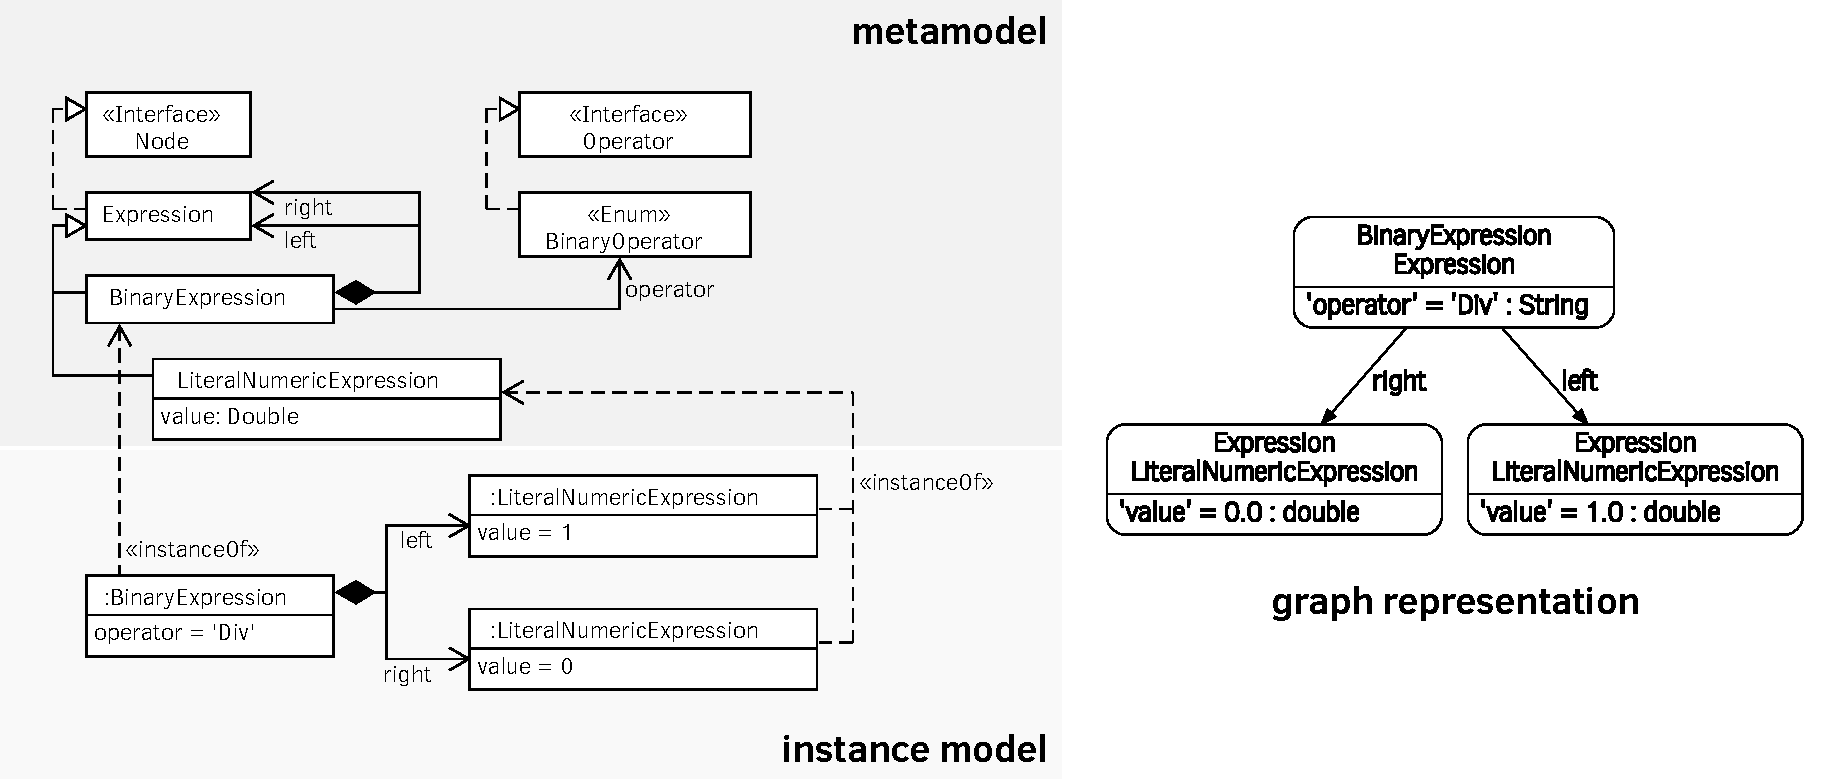
\includegraphics[width=\textwidth]{object-to-graph.pdf}
  \caption{Transformation of a Java object structure into a graph.}
  \label{fig:object-to-graph}
\end{figure}

In order to acquire information from this model and transform it, one either knows its metamodel and iterates over every element or --- if the programming language of the parser allows --- uses reflection. In my approach I use the combination of the Shift parser written in Java --- thus using the reflective approach --- and the Neo4j labeled property graph database.

\paragraph{Typed Nodes}
Every AST or ASG node is a node in the graph. The graph node is typed with the class, superclasses and interfaces of the represented model entity.

% CFG end node is also created for every node

\paragraph{Node Properties}
Every property of a model entity --- regardless of whether they are its own or inherited from its supertypes --- are also transferred to the graph node. These properties are also stored with their basic type: \emph{double}, \emph{string} or \emph{boolean}.

\paragraph{Labeled Relations}
References in the model are represented in the graph as relations, directed edges. The relations are labeled after the name of the references.

\paragraph{Collections}
The metamodel also contains several reference collections: maps, lists and tables. Maps and tables are represented in the graph as a new node, with appropriately labeled relations to the referred nodes.

Lists are transformed similarly. In order not to lose ordinal information, the items are related to the referrer with two routes (see~\Cref{fig:graph-list}).

\begin{figure}[!htb]
  \centering
  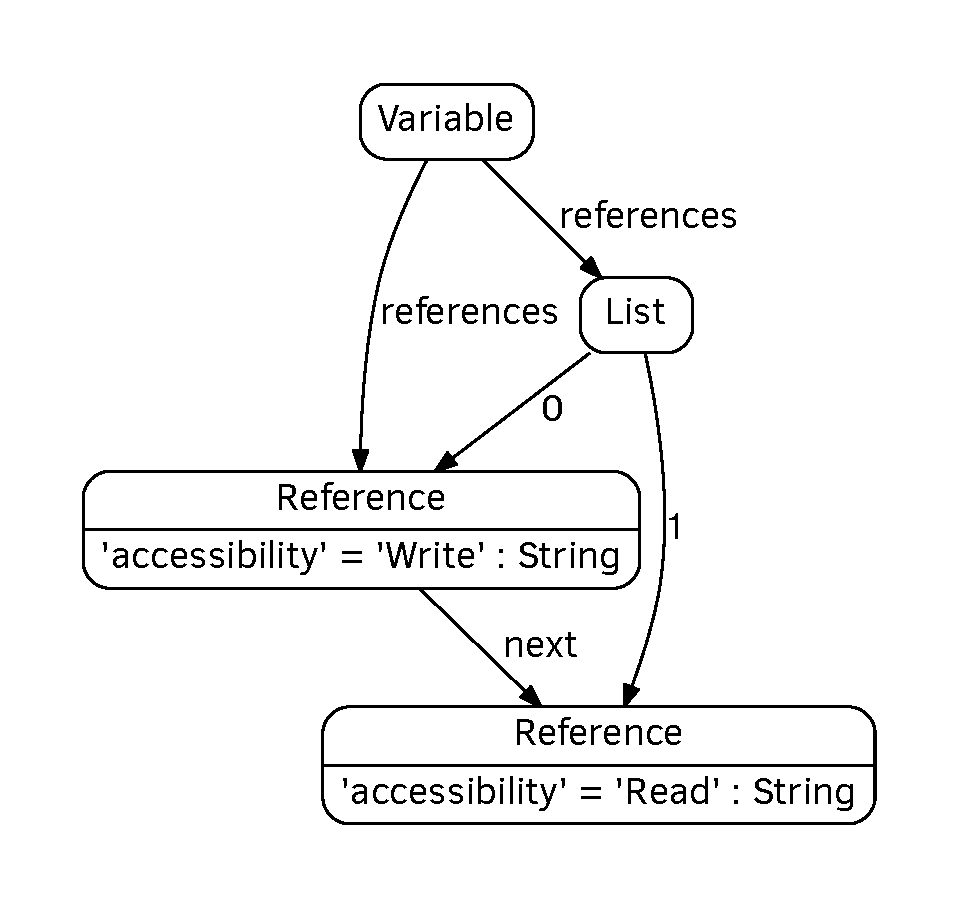
\includegraphics[width=0.5\textwidth]{graph-list.pdf}
  \caption{Graph Representation of a List}
  \label{fig:graph-list}
\end{figure}

The first route is direct; the referrer has a relation to every item of the list (labeled with the name of the list). The second route has an additional \emph{List} node between the two, and its relations are labeled with the index of the item. The sequential items also have a direct, chaining relation.

% last item of the list is marked
%\paragraph{Functional Elements}

\paragraph{Source Code Location}
To be able to report precise location for a problem, the graph also contains line and character information for the beginning and the end of every model entity.


\subsubsection{Storing the Graph Representation}
If the parser successfully processes the source code, the resulting ASG is transformed with the forementioned rules. In a writing transaction, the transformed graph is serialized and stored in the database.

\paragraph{Metadata}
Besides the ASG, additional properties are stored. For example, for every source file, a node exists in the graph connected to nodes belonging to the particular ASG. This makes it easier to handle nodes of a file as a whole.

\paragraph{Multilayered Graph}
With more complex rules it is also feasible to store multiple versions of the same file in the database. This makes it possible to maintain multilayered versioning for multiple users.

If the VCS supports branching the code development, the framework could also accomodate this behaviour. For example if two developers work on the \emph{master} development branch in their own IDE, there could be layers for each of them.

\begin{figure}[!htb]
  \centering
  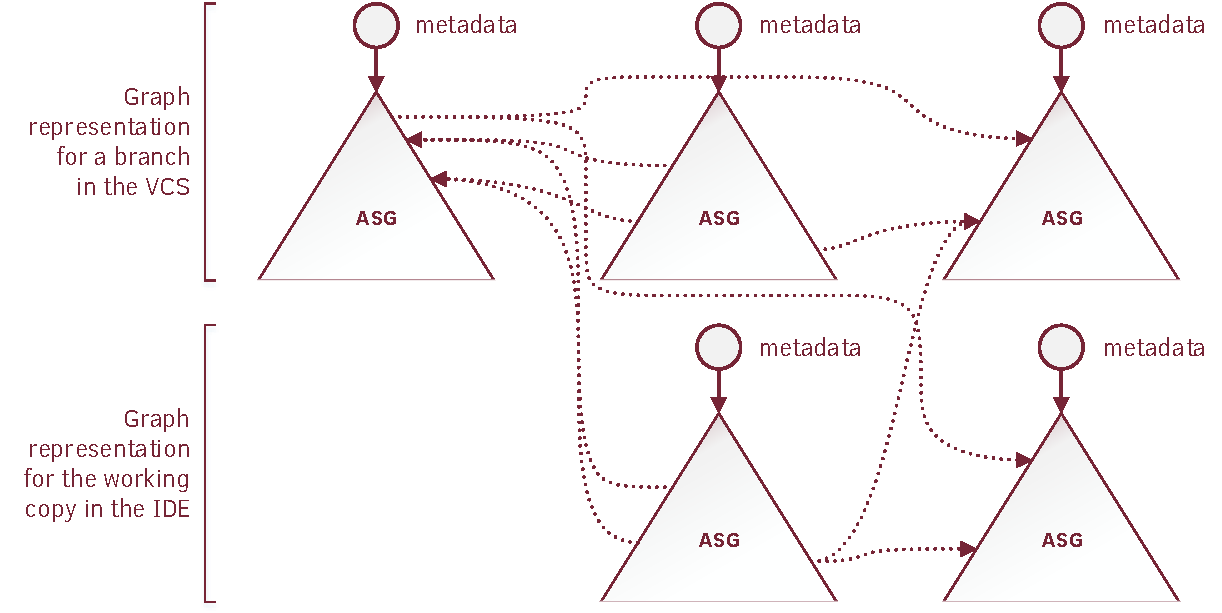
\includegraphics[width=\textwidth]{multilayer.pdf}
  \caption{Multilayered graph.}
  \label{fig:multilayered-graph}
\end{figure}

One layer containing every ASG for the \emph{master} branch. One layer for each user containing only the ASGs of their modified files. In these layers the ASGs are connected (based on the import and export statements) in the same layer, if both are present in the same. If not, they are connected to the corresponding file in the \emph{master} branch (see~\Cref{fig:multilayered-graph}).

\subsubsection{Transforming the Graph}
After the data has been stored in the database, it can be freely transformed with framework- or user-defined rules. This step may be utilized for transforming the set of subgraphs into one connected graph based on the export and import rules of the language (detailed in~\Cref{sect:handling-import-export}).

Neo4j makes it possible to execute in-place transformations, where querying with pattern matching and manipulations may be declared in the same query. The possibilities of Neo4j are detailed in~\Cref{sect:neo4j}. Transformation examples are presented and visualized in~\Cref{chap:elaboration-of-the-workflow}.

\subsection{Executing Graph Queries}
By utilizing the built-in pattern-matching abilities of Neo4j, it is easier and more user-friendly to write pseudo-graphic, declarative patterns to find a structure in the graph --- compared to the generally used visitor patterns.~\cite{csmr} An example graph pattern query is detailed in~\Cref{sect:division-by-zero}.

If the query language of Neo4j, Cypher is not powerful enough to express logic in a standalone query, one may also utilize arbitrary Java code. This code may be used inside the query or even command multiple queries and aggregate the result.
